% TEMPLATE for Usenix papers, specifically to meet requirements of
%  USENIX '05
% originally a template for producing IEEE-format articles using LaTeX.
%   written by Matthew Ward, CS Department, Worcester Polytechnic Institute.
% adapted by David Beazley for his excellent SWIG paper in Proceedings,
%   Tcl 96
% turned into a smartass generic template by De Clarke, with thanks to
%   both the above pioneers
% use at your own risk.  Complaints to /dev/null.
% make it two column with no page numbering, default is 10 point

% Munged by Fred Douglis <douglis@research.att.com> 10/97 to separate
% the .sty file from the LaTeX source template, so that people can
% more easily include the .sty file into an existing document.  Also
% changed to more closely follow the style guidelines as represented
% by the Word sample file. 

% Note that since 2010, USENIX does not require endnotes. If you want
% foot of page notes, don't include the endnotes package in the 
% usepackage command, below.

\documentclass[letterpaper,twocolumn,10pt]{article}
\usepackage{epsfig,endnotes}
\usepackage{usenix-2020-09}
\usepackage{kotex}
\usepackage{graphicx}
\usepackage{subfig}
\usepackage{xcolor}
\usepackage{comment}
\usepackage[numbers,sort&compress]{natbib}
%\usepackage[breaklinks]{hyperref}
\def\UrlBreaks{\do\/\do-}

\newcommand{\BSK}[1]{\textcolor{red}{#1}}
\newcommand{\EUNJI}[1]{\textcolor{blue}{#1}}
\newcommand{\FOOTBF}[1]{\footnotesize{\bf{#1}}}
\newcommand{\WHERETOGO}[1]{\textcolor{orange}{WHERETOGO: #1}}
\newcommand{\ours}{\texttt{Dawid}}

\begin{document}

%don't want date printed
\date{}

%make title bold and 14 pt font (Latex default is non-bold, 16 pt)
% \title{\Large \bf Wonderful : A Terrific Application and Fascinating Paper}
% \title{\Large \bf Dawid: A Cost-effective I/O Scheduling Scheme for SSDs under Capacitance Constraints}
% \title{\Large \bf Least Increase of Dirtiness Scheduling for SSDs under Capacitance Constraints}
\title{\Large \bf Overcoming Capacitance Constraints in SSD}
% \author{
% {\rm Sanghyun Nam$^\dagger$, Seungmin Shin$^\dagger$, Sungjin Lee$^\ddagger$, Bryan S. Kim$^\ast$, Eunji Lee$^\dagger$}\\
% Soongsil University$^\dagger$, DGIST$^\ddagger$, Syracuse University$^\ast$
% }
\author{
{\rm Sanghyun Nam}\\
Soongsil University
\and
{\rm Seungmin Shin}\\
Soongsil University
\and
{\rm Sungjin Lee}\\
DGIST
\and
{\rm Bryan S. Kim}\\
Syracuse University
\and
{\rm Eunji Lee}\\
Soongsil University
}
\maketitle

% Use the following at camera-ready time to suppress page numbers.
% Comment it out when you first submit the paper for review.
\thispagestyle{empty}

% \subsection*{Abstract}
% Enterprise-class SSDs realize a persistent buffer within device using the capacitors. 
% This approach reached a limit as the SSD density outpaces the scaling capability of the capacitors. 
% This paper presents a novel buffer architecture for SSDs under capacitance constraints. 
% We re-order the write requests in a way of minimizing the memory footprint 
% that needs protection. 
% % such that the number of dirty pages within buffer
% % is minimized at a time window. 
% This design reduces the required capacitance to ensure persistence in SSDs 
% at the modest performance loss. 
% % This design significantly mitigates the additional flash writes 
% % wherein the capacitors protect a portion of the buffer. 
% % caused by the limits of capacitance.
% \EUNJI{
% We implemented \ours{} in an open-source SSD development 
% framework. Performance evaluation shows that \ours{} has only 10\% more flash writes 
% than full-protection SSD, while the required capacitence is reduced by 70\%.
% }
% capacitance limitation of SSD. 
%SSD density scales up at the fast pace, but other components keep up with the speed. 

% 배터리로 보호를 덜하지만 
% ==> 사실 스파르탄이랑 합칠 수 있을 듯.
% ==> DuraSSD 같은 거임. 맵핑 테이블이 업데이트 되었는데 한계치를 넘지 못할 때 
% ==> dirty page 의 숫자를 가능하면 줄여서 성능을 높이고 


% 배터리로 모두 보호되던 SSD buffer 는 face the limitation. 
% dirty pages 의 수가 제한된 상황에서 플래시 메모리로 보내지는 쓰기량을 절감할 수 있는 기법을 제안. 

% 맵핑 테이블 vs. 사용자 데이터 
% ==> 맵핑 테이블의 flush 가 발생시키는 트래픽의 비중이 얼마나 되나? 
% \vspace{-100pt}
%%\vspace{-20pt}
\section*{Abstract}
The growth in SSD capacity is reaching its limit 
due to the stunted growth of capacitors---electrical components that store charge 
to protect data for the volatile memory in case of power loss. 
While the SSD's capacity scaled from 256GB in 2011~\cite{samsung2011} to 30TB in 2018~\cite{anandtech18samsung} (100$\times$), 
the density of Aluminum and Tantalum electrolytic capacitors only by tenfold from 1960 to 2005~\cite{both2015modern}.
This slow scaling will eventually limit the amount of DRAM that can be used in an SSD,
and this, in turn, will also limit the storage capacity as the size of DRAM and aggregate flash capacity proportionally scale~\cite{samsung_ratio, ni2017hash}. 

\iffalse
Enterprise-class SSDs provide a persistent internal buffer using the capacitors. 
This PLP(Power-Loss Protection) mechanism reached a limit as the SSD density outpaces the scaling capability of the capacitors. 
% The SSD has increased significantly in density for the past decade. 
% With the growing popularity of data-intensive applications, the SSD density has increased rapidly in recent years.
%, expanding by 100× over the past ten years [1], [15].
% As an example, 
In 2011, a typical 2.5-inch SSD had 256GB capacity, but
%the world's first 2TB SSD was released in 2013~\cite{foremay2013}, but 
by 2018, a high-capacity SSD boasted a 30TB, expanding by 100× over the past ten years
~\cite{samsung2011, anandtech18samsung}. 
\begin{comment}
This remarkable growth of the device-capacity is thanks to the advanced scaling technologies 
such as nanoscale fabrication~\cite{busche2014design} and multi-layer stacking~\cite{9365809}. 
\end{comment}
% As an example, in 2011, a typical 2.5-inch SSD had 256GB capacity with 256MB of DRAM; by 2018, a high-capacity 2.5- inch SSD boasted a 30TB with 40GB of
% Unfortunately, not all components of the SSDs have kept up with the scaling rate.
However, the capacitor fails to proceed at the pace. 
\begin{comment}
Historically, storage devices 
have been equipped with a small size of volatile buffer in front of the persistent disk. 
By using them as a write buffer, they hide a long latency of the physical storage medium 
as well as mitigating an endurance limitation of the worn-out devices. 
However, the volatile buffer loses all data in the event of power crash. 
To prevent a data loss or corruption by this, enterprise-class SSDs
rely on the capacitors; it reserves energy to persist data in volatile buffer 
in the unforeseen event of a power crash. 
In addition, the adoption of capacitors enables an SSD to ignore the \texttt{FLUSH} command that explicitly requests all data in the volatile buffer to be made durable.
This property increases the buffering effect in SSD significantly, leading to both less write traffic and a shorter operation latency.
% To overcome this limitation without sacrificing performance, 
The reliance on capacitors, however, has reached its limit. 
\end{comment}
% the improvement in capacitance fails to keep up with the rapid growth of SSDs. 
%Al(aluminum) and Ta(tantalum)-electrolytic capacitors used in SSDs have increased in density through miniaturization by tenfold from 1960 to 2005 [4]. 
The capacitance density has also steadily improved, but
it is not as rapid as the SSD scaling speed. 
Al(aluminum) and Ta(tantalum)-electrolytic capacitors used in SSDs 
have increased in density by tenfold from 1960 to 2005~\cite{both2015modern}. 
This is approximately 50x slower than the SSD density increase rate.
Given that the internal buffer size increases in proportion to the storage capacity (typically 0.1\% of storage capacity~\cite{samsung_ratio, ni2017hash}),
the density gap between capacitance and memory technologies 
imposes an intrinsic limitation on the current architecture wherein 
the entire buffer is protected by capacitors. 
\fi

This paper presents \ours{}, a novel SSD-internal DRAM management scheme 
that allows the SSD capacity to scale beyond the slow growth of capacitors. 
SSD-internal DRAM is used for 
(1) caching translation information (also known as mapping table) and (2) buffering user writes. 
In typical SSD designs, most of the capacitance is used for protecting the mapping table (to keep as many translation entries in DRAM) 
and the buffer for user writes is kept at a minimal (just enough to hide the flash program latency)~\cite{KangLMKO14sigmod}. 
However, in our design, we take a radically different approach. 
We buffer more user writes so that mapping entry eviction becomes more efficient by aggregating dirty updates. 
This substantially reduces the amount of mapping table-related write traffic, and in turn, improves the overall performance. 

\iffalse
This paper presents a device-internal buffer architecture called \ours{} 
for the SSDs under capacitance constraints. 
% which operates under capacitance constraints.
% Fig.~\ref{fig_dawid_archi} shows the SSD architecture targeted in our study. 
\fi
\iffalse
\textcolor{blue}{
Historically, storage devices have been equipped with a small size of volatile buffer in front of the persistent disk. By using them as a read cache and a write buffer, they hide a long latency of the physical storage medium as well as mitigating an endurance limitation of the worn-out devices.
However, the volatile buffer loses all data in the event of power crash. 
To prevent a data loss or corruption by this, enterprise-class SSDs
rely on the capacitors; it reserves energy to persist data in volatile buffer 
in the unforeseen event of a power crash. 
In addition, the adoption of capacitors enables an SSD to ignore the \texttt{FLUSH} command that explicitly requests all data in the volatile buffer to be made durable.
This property increases the buffering effect in SSD significantly, leading to both less write traffic and a shorter operation latency.
% \EUNJI{Need to make this part shorter}
}
\fi
% To overcome this limitation without sacrificing performance, 
% The reliance on capacitors, however, has reached its limit. 
\iffalse
\ours{} achieves a persistent buffer with small size of capacitance by answering the following two questions. 
%(1) what not to protect under capacitance limitation and (2) how to reduce the overhead of ensuring persistence for unprotected data.
First question is \textit{what not to protect under capacitance constraints}. The device-internal buffer is used for (1) caching translation information (i.e., mapping index) and (2) buffering user writes. 
% The data maintained in the buffer can be classified into two types: the actual user data and 
% the metadata for SSD management (i.e, mapping table). 
\ours{} applies the capacitance constraints only to translation information, while protecting the user data entirely. The user data write is synchronous with the user request and unrecoverable upon a power outage. It hampers user experiences seriously when unprotected. On contrary, 
translation information is entirely managed by the firmware and provides room for compromise when SSDs suffer from capacitance restriction. \EUNJI{Furthermore, the main culprit demanding buffer space is translation information because a flat structured table is widely used for its indexing and has a large memory footprint.} 
Second question is thus \textit{how to reduce the cost of ensuring persistence for the translation updates}. When the buffer is partially protected, the number of dirty pages is limited to the maximum amount of data that the on-board capacitance can protect. If it goes beyond the limit, changes should be immediately flushed to the flash memory. \ours{} mitigates the negative impact of this behavior with a capacitance-contraint aware I/O scheduling.
%to meet the durability constraint for SSDs. XX mapping table XX flush 줄여보자.

% otherwise durability violated. 
% \EUNJI{
% 보호되지 못하는 데이터가 있을 때 버퍼를 어떻게 관리하면, 보호되지 못하는 데이터의 persistence 를 유지하기 위해 발생하는 비용을 적게 발생시킬 것인가? 에 대한 질문. }
% \EUNJI{제안하는 기법: 부분적으로 보호되는 맵핑 테이블의 동기화 오버헤드를 줄이기 위해, 해당 비용을 최소로 증가시키도록 I/O 스케줄링을 하는 것임.}
\fi
%\section{Design of \ours{} Buffer}
% \section{Least Increase of Dirtiness Scheduling}
\iffalse
A primary way of  reducing the superfluous writes caused by a capacitance limitation is to maintain the dirty memory footprint below a protected threshold as long as possible. When a dirty page overflow occurs, flushing is forced and write amplification increases.
% The \ours{} buffer aims at minimizing the dirty memory footprint of the mapping table at any point in time.
To this end, \ours{} aggregates and batches the requests whose mapping entry resides in the same page. This policy reduces the dirty memory footprint of the mapping table at any point in time, amortizing the synchronization overhead across more requests. As such, \ours{} delivers less write traffic and higher IOPS than existing scheduling (e.g., FIFO) under capacitance constraints. 
\fi

To realize this design, 
\ours{} maintains two data structures: first, \textit{a zero-cost list} 
that holds the write requests whose mapping entry is already in a dirty translation page, 
and second, \textit{a max binary heap} that maintains the indexes to translation pages
sorted by the number of buffered user write requests associated with that page. 
% We term this policy Least Increase of Dirtiness (LID) scheduling.
When there is sufficient bandwidth at underlying NAND flash subsystem for writes, 
\ours{} first flushes user data from the  zero-cost list,
and then persists the dirty translation pages as ordered by the max binary heap. 
By doing so, each user write minimizes the number of eventual translation page write, 
and each translation page write maximizes the number of persisted mapping entries. 
\iffalse
\BSK{What's policy on the maximum number of dirty translation pages? Dawid should also flush when that condition satisfies, right?}
\EUNJI{FIFO로 flush 합니다. SSD 가 한번에 병렬적으로 쓸 수 있는 단위씩 보냅니다.}
\fi
 

\iffalse
In this regard, the \ours{} buffer aims at minimizing the \textit{dirty memory footprint} of the mapping table at any point in time. To this end, \ours{} processes outstanding requests in the order that least increases the number of dirty pages in the mapping table. 
This scheme not only reduces the number of flushes for the mapping table partially protected but also increases the efficiency of flush operation by aggregating more translation updates into the smaller translation pages.
\fi

\iffalse
because (1) the data write is synchronous with the user request and (2) the user data takes up a relatively 
small footprint in the buffer. 
\fi
% This is because the storage suffers from serious performance degradation when the user data 
% is not fully protected and should be entirely flushed upon a \texttt{FLUSH} command.
% }
% \textcolor{brown}{
% \ours{} essentially limits the number of dirty pages within buffer
% to the level the maximum capacitance can protect.
% If the number of dirty pages goes beyond the limit, changes are flushed to the flash memory. 
% }
% \EUNJI{For this architecture, the problem boils down to how to reduce the write traffic to persist the mapping table to flash memory under capacitance constraints.
% \iffalse
\iffalse
Reducing the synchronization overhead of the mapping table is a well-known problem and has been extensively studied for a past decade~\cite{jiang2011s, kim2017shrd}. 
However, they mostly focus on the SSDs without PLP, which have different properties to the PLP-SSDs with capacitance constraints. 
\fi

\ours{} is built upon the current trend of increasing the queue depth of the storage interfaces. SATA and SAS support a single queue with 32 and 245 commands, but NVMe has 
up to 65,535 queues with as many as 65,536 commands per queue. 
This extension allows SSDs to further optimize the internal activities by taking advantage of the outstanding request information.


\begin{figure}[t]
    \centering{}
    \subfloat[Write Traffic] {
	    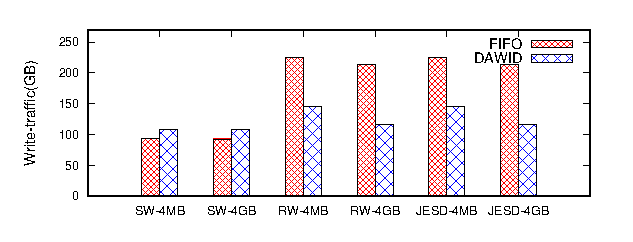
\includegraphics[width=0.4\textwidth]{figure/all-wt.eps}
	} \\
	\subfloat[IOPS] {
	    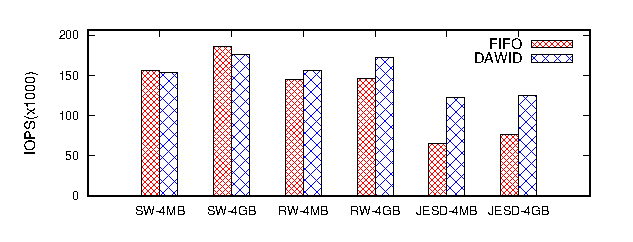
\includegraphics[width=0.4\textwidth]{figure/all-iops.eps}
	}
	\caption{Fio benchmark results.}
	\label{fig_fio}
\end{figure}

We implement \ours{} in \texttt{FEMU}, an open-source SSD development framework~\cite{li2018case}.
We assume 1\% of the mapping table is protected via capacitors in a 64GB SSD. 
%The 64GB SSD is using DRAM and assumes that 1\% of the mapping table is protected. 
We measured the performance of \ours{} using fio benchmark~\cite{fio-bench},
running 4KB sequential writes, 4KB random writes, 
and the skewed read-write mixed workload that follows JESD219 using 8 threads. 
A total of 90GB of data was written to the 30GB area.

\EUNJI{
Figure~\ref{fig_fio} compares IOPS and the write traffic of FIFO buffer management and \ours{}.
For sequential writes, there are no prominent differences between FIFO and \ours{}. 
However, \ours{} reduces the write traffic by 35\% and 46\% on average 
for random writes and JESD219 workloads when the buffer size is 4MB and 4GB, respectively. 
These workloads have a large footprint at a time window and thus buffering and scheduling them judiciously leads to a large reduction in mapping table persistence overhead.
Consequently, IOPS of our design improves up to 18\% and 88\% for random write and JESD219, respectively.
}

% \EUNJI{
% To extending this work, we plan to investigate the trade-offs between performance and capacitance.
% }

\iffalse
To evaluate the effectiveness of \ours, we implement the proposed buffer design
in \texttt{FEMU}, which is an open-source SSD development framework~\cite{li2018case}. The performance evaluation with various workloads 
shows that \ours{} reduces the write traffic by up to 78\% and provides 25\% higher IOPS 
compared to the FIFO scheduling scheme when only 10\% of the mapping table is protected. 
Compared to the full-protection architecture, \ours{} has has 20\% more writes and 
9\% of performance overhead, while reducing the required capacitance by 90\%. 
\fi

% \begin{figure}[t]
%     \centering{}
%     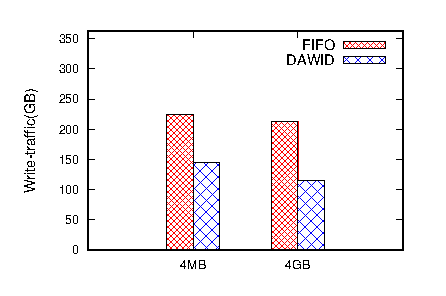
\includegraphics[width=0.20\textwidth]{shn-graph/rand-wt.eps}
%     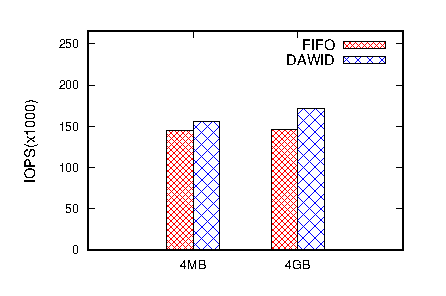
\includegraphics[width=0.20\textwidth]{shn-graph/rand-iops.eps}
%     %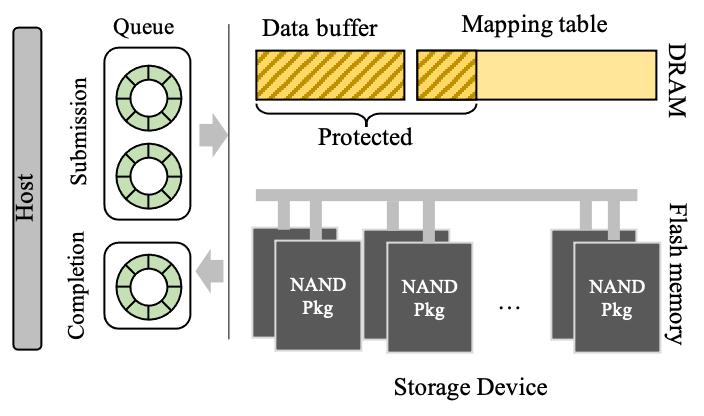
\includegraphics[width=0.4\textwidth]{figure/dawid_ssd_archi.png}
%     \caption{\textbf{Write Traffic and IOPS (FIO-RAND).}}
%     \label{fig_dawid_archi}
% \end{figure}

% \begin{figure}[t]
%     \centering{}
%     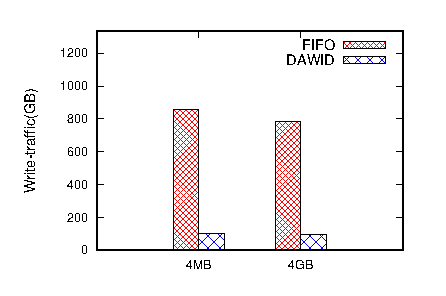
\includegraphics[width=0.20\textwidth]{shn-graph/jesd-wt.eps}
%     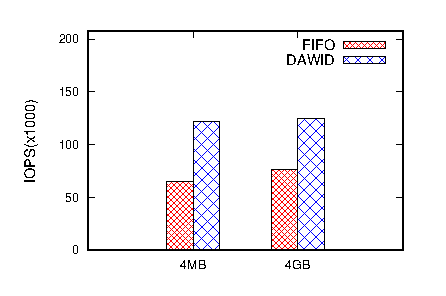
\includegraphics[width=0.20\textwidth]{shn-graph/jesd-iops.eps}
%     %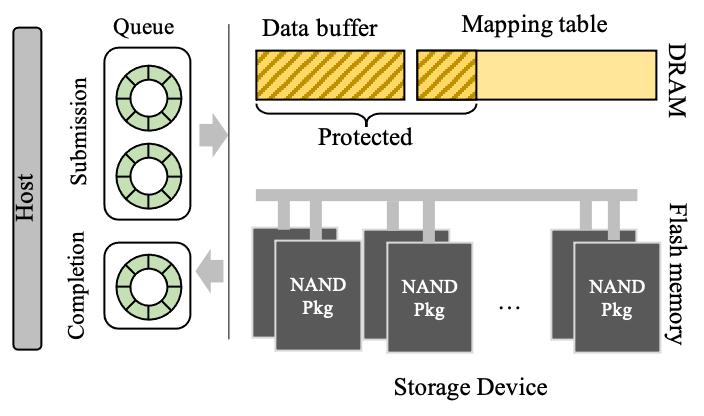
\includegraphics[width=0.4\textwidth]{figure/dawid_ssd_archi.png}
%     \caption{\textbf{Write Traffic and IOPS (FIO-JESD) .}}
%     \label{fig_dawid_archi}
% \end{figure}


\section*{Abstract}
The growth in SSD capacity is reaching its limit 
due to the stunted growth of capacitors---electrical components that store charge 
to protect data for the volatile memory in case of power loss. 
This paper presents \ours{}, a novel SSD-internal DRAM management scheme 
that allows the SSD capacity to scale beyond the slow growth of capacitors. 
\ours{} suppresses an increase of the dirty memory footprint within buffer 
using the deep queues available in today's storage interfaces.
We implement our design in \texttt{FEMU}, an open-source SSD development framework
and demonstrate that \ours{} delivers IOPS close to 90\% of performance at only 1\% of capacitance compared to the existing scheme. 

\section{Introduction}

% Unfortunately, not all components of the SSDs have kept up with the scaling rate.
% The capacitor, which is adopted in enterprise-class SSDs for power-loss protection (PLP), fails to proceed at the pace. Historically, storage devices 
% have been equipped with a small size of volatile buffer in front of the persistent disk. 
% By using them as a read cache and a write buffer, they hide a long latency of the physical storage medium 
% as well as mitigating an endurance limitation of the worn-out devices. 
% However, the volatile buffer loses all data in the event of power crash. 
% To prevent a data loss or corruption by this, enterprise-class SSDs
% rely on the capacitors; it reserves energy to persist data in volatile buffer 
% in the unforeseen event of a power crash. 
% In addition, the adoption of capacitors enables an SSD to ignore the \texttt{FLUSH} command that explicitly requests all data in the volatile buffer to be made durable.
% This property increases the buffering effect in SSD significantly, leading to both less write traffic and a shorter operation latency.

% \EUNJI{Historically, storage devices 
% have been equipped with a small size of volatile buffer in front of the persistent disk. 
% By using them as a read cache and a write buffer, they hide a long latency of the physical storage medium 
% as well as mitigating an endurance limitation of the worn-out devices.}
The enterprise-class SSDs adopt the capacitor to protect data durability in case of power crash. 
This technique is called Power-Loss Protection (PLP)~\cite{micron2014, intel2014, samsungplp2016} and it is needed because SSDs use a DRAM as an internal buffer for absorbing user writes and caching translation information (also known as mapping table). 
If they are not protected, SSDs will have not only a data loss and/or corruption but also a long recovery time to build an up-to-date  mapping table by scanning entire flash drives.
To preclude this situation, the enterprise-class SSDs rely on the capacitors that reserve energy to safely persist data of the volatile buffer in a power loss.
\textcolor{orange}{
Table I summarizes the policies for power loss protection (PLP) across several SSDs. While client SSDs such as the Samsung 950Pro and Micron M5001 forgo PLP, enterprise SSDs use capacitors that supply enough energy during powerloss to persist all data in the volatile memory to a temporary location in flash.
(EJ: ISLPED 논문에서 긁어와서 좀 바꿔야 할듯..)
}
% In addition, the adoption of capacitors enables an SSD to ignore the \texttt{FLUSH} command that explicitly requests all data in the volatile buffer to be made durable.
% This property increases the buffering effect in SSD significantly, leading to both less write traffic and a shorter operation latency.

% The SSD-internal volatile buffer loses all data in the event of power crash. 
% To prevent a data loss or corruption by this, enterprise-class SSDs
% rely on the capacitors; it reserves energy to persist data in volatile buffer 
% in the unforeseen event of a power crash.
% In addition, the adoption of capacitors enables an SSD to ignore the \texttt{FLUSH} command that explicitly requests all data in the volatile buffer to be made durable.
% This property increases the buffering effect in SSD significantly, leading to both less write traffic and a shorter operation latency.

% To overcome this limitation without sacrificing performance, 
However, the heavy reliance on capacitors is no longer sustainable as the increase in SSD far outpaces 
the increase in capacitor density.
The SSD has increased significantly in density for the past decade. 
In 2011, a typical 2.5-inch SSD had 256GB capacity, but
%the world's first 2TB SSD was released in 2013~\cite{foremay2013}, but 
by 2018, a high-capacity SSD boasted a 30TB, expanding by 100× over the past ten years
~\cite{samsung2011, anandtech18samsung}. 
This remarkable growth of the device-capacity is thanks to the advanced scaling technologies 
such as nanoscale fabrication%~\cite{busche2014design}
and multi-layer stacking. %~\cite{9365809}. 
Al(aluminum) and Ta(tantalum)-electrolytic capacitors used in SSDs 
have increased in density by tenfold from 1960 to 2005. 
This is approximately 50x slower than the SSD density increase rate.
Given that the internal buffer size increases in proportion to the storage capacity~\cite{ni2017hash},
the slow scaling of capacitors will eventually limit the amount of DRAM that can be used in an SSD. 
This, in turn, will also limit the storage capacity as the size of DRAM and aggregate flash capacity proportionally scale. 
% ~\cite{samsung_ratio, ni2017hash}

\iffalse
the density gap between capacitance and memory technologies 
imposes an intrinsic limitation on the current architecture wherein 
the entire buffer is fully protected by capacitors. 
\fi
% \begin{figure}[t]
%     \centering{}
%     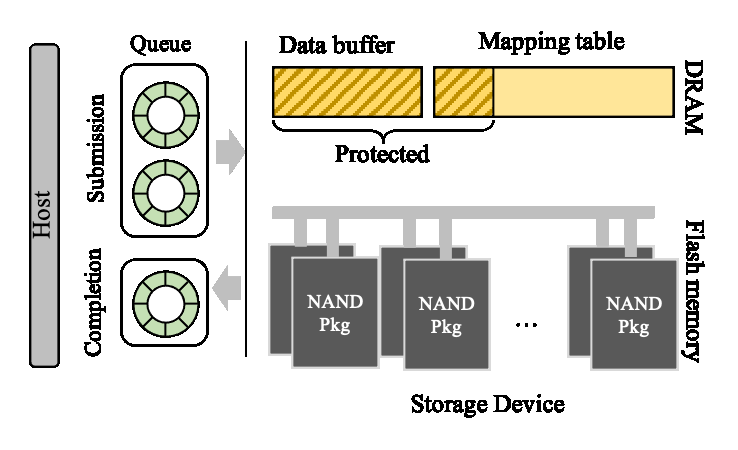
\includegraphics[width=0.4\textwidth]{figure/dawid_ssd_archi.eps}
%     %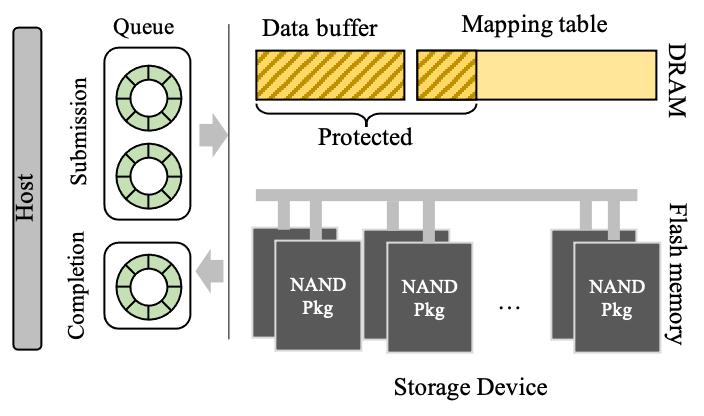
\includegraphics[width=0.4\textwidth]{figure/dawid_ssd_archi.png}
%     \caption{\textbf{SSD architecture with \ours{} buffer.}}
%     \label{fig_dawid_archi}
% \end{figure}
% \EUNJI{to scale ...}

% This paper presents a device-internal buffer architecture called \ours{}
% for the SSDs under capacitance constraints. \ours{} only XXX. 

\iffalse
This paper presents \ours{}, a novel SSD-internal DRAM management scheme 
that allows the SSD capacity to scale beyond the slow growth of capacitors. 
SSD-internal DRAM is used for 
(1) caching translation information (also known as mapping table) and (2) buffering user writes. 
In typical SSD designs, most of the capacitance is used for protecting the mapping table (to keep as many translation entries in DRAM) 
and the buffer for user writes is kept at a minimal (just enough to hide the flash program latency)~\cite{KangLMKO14sigmod}. 
% As an example, Samsung PM1643 30.72TB and PM1633a 15.36TB house 40GB and 16GB DRAM, respectively~\cite{anandtech18samsung}. 
% (typically 0.1\% of storage capacity~\cite{samsung_ratio, ni2017hash})
\fi
This paper presents \ours{}, a novel SSD-internal DRAM management scheme 
that allows the SSD capacity to scale beyond the slow growth of capacitors. 
SSD-internal DRAM is used for 
(1) caching translation information (also known as mapping table) and (2) buffering user writes. 
In typical SSD designs, most of the DRAM is used for caching the mapping table and 
and the buffer for user writes is kept at a minimal (just enough to hide the flash program latency)~\cite{KangLMKO14sigmod}. 
% As an example, Samsung PM1643 30.72TB and PM1633a 15.36TB house 40GB and 16GB DRAM, respectively~\cite{anandtech18samsung}. 
% (typically 0.1\% of storage capacity~\cite{samsung_ratio, ni2017hash})


% As an example, Samsung PM1633a 15.36TB SSD houses 16GB DRAM~\cite{anandtech18samsung}. 
% Given that the mapping table size is typically 0.1\% of storage capacity~\cite{samsung_ratio, ni2017hash}, 
% we can assume that only 4\% of DRAM is used for a write buffer. 

\begin{table}[b]
    \centering
    \fontsize{11}{11}
    \small
	% Model Manufacturer Category PLP-Support Capacitor 
    %\begin{tabular}{p{2.4cm}|p{1.3cm}|p{1.2cm}|l}
    %\begin{tabular}{p{2.4cm}|p{2.4cm}|p{2.4cm}|p{2.4cm}|p{2.4cm}}
    \begin{tabular}{|l|l|l|l|l|}
        \hline
        \footnotesize{\bf{SSD Model}} &
        \footnotesize{\bf{Manufacturer}} & 
        \footnotesize{\bf{Class}} &
        \footnotesize{\bf{PLP}} & 
        \footnotesize{\bf{Capacitor}} \\ \hline \hline

        \footnotesize{950Pro, 850Pro} & \footnotesize{Samsung} & \footnotesize{Client} & \footnotesize{None} & - \\ \hline
        \footnotesize{M500} & \footnotesize{Micron} & \footnotesize{Client} & \footnotesize{Partial} & \footnotesize{Ceramic} \\ \hline
        \footnotesize{M500DC} & \footnotesize{Micron} & \footnotesize{Enterprise} & \footnotesize{Full} & \footnotesize{Tantalum} \\ \hline
        \footnotesize{PM863, SM863} & \footnotesize{Samsung} & \footnotesize{Enterprise} & \footnotesize{Full} & \footnotesize{Tantalum} \\ \hline
        \footnotesize{DC1000B} & \footnotesize{Kingston} & \footnotesize{Enterprise} & \footnotesize{Full} & \footnotesize{Tantalum} \\ \hline
        \footnotesize{DC S3700, S3500} & \footnotesize{Intel} & \footnotesize{Enterprise} & \footnotesize{Full} & \footnotesize{Aluminum} \\ \hline
    \end{tabular}
    \caption{\textbf{Power Loss Protection in SSDs~\cite{micron2014, intel2014, samsungplp2016}}.}
    \label{ssd_plp}
    \vspace{-20pt}  
\end{table}
\iffalse
\textcolor{red}{
As opposed to a memory pressure, the negative impact of data loss is equally serious for both data. Because an SSD writes the associated LPN (Logical Page Number) in the OOB (Out-of-band) area of the physical page, it is virtually possible to recover the up-to-date mapping table by scanning the entire NAND flash memory. However, because it takes prohibitively long, particularly for the scalable SSDs, PLP-SSD snapshots an entire mapping table into the specific area in NAND flash in a power loss and loads it into DRAM at a reboot. The user data also offers no alternative but for PLP as it cannot be recovered after a crash. For the PLP-SSD, the host system ensures reliability assuming that all acknowledged data survive a power outage, and thus, the loss of user data can lead to a catastrophic result.
}
\fi

% \ours{} applies this compromise only to the metadata, while protecting the user data entirely. 
% The data write is not only synchronous with the user request, which hampers user experiences seriously when delayed, but also unrecoverable in the event of the power crash. 

\textcolor{orange}{However, in our design,
we take a radically different approach. \ours{} protects a fraction of the mapping table. 
We buffer more user writes so that mapping entry eviction becomes more efficient
by aggregating dirty updates. This substantially reduces the
amount of mapping table-related write traffic, and in turn,
improves the overall performance.}
%  and persists changes to a NAND flash memory if the dirty memory footprint overflows. 
% while fully protecting the user data. 
% \textcolor{orange}{The write latency of user data affects user experience significantly,
% it is hard to compromise it for reducing capacitance.}
% Instead, \ours{} buffers more user writes so that mapping entry eviction becomes more efficient by aggregating dirty updates. 
% This substantially reduces the amount of mapping table-related write traffic, and in turn, improves the overall performance under capacitance constraints. 

To realize this design, 
\ours{} maintains two data structures: first, \textit{a zero-cost list} 
that holds the write requests whose mapping entry is already in a dirty translation page, 
and second, \textit{a max binary heap} that maintains the indexes to translation pages
sorted by the number of buffered user write requests associated with that page. 
% We term this policy Least Increase of Dirtiness (LID) scheduling.
When there is sufficient bandwidth at underlying NAND flash subsystem for writes, 
\ours{} first flushes user data from the  zero-cost list,
and then persists the dirty translation pages as ordered by the max binary heap. 
By doing so, each user write minimizes the number of eventual translation page write, 
and each translation page write maximizes the number of persisted mapping entries. 


\ours{} is built upon the current trend of increasing the queue depth of the storage interfaces. SATA and SAS support a single queue with 32 and 245 commands, but NVMe has 
up to 65,535 queues with as many as 65,536 commands per queue. 
This extension allows SSDs to further optimize the internal activities by taking advantage of the outstanding request information.

We implement \ours{} in \texttt{FEMU}, an open-source SSD development framework~\cite{li2018case}.
The performance evaluation with various workloads shows that \ours{} offers 82\% and 94\% of IOPS of the full-protection SSD when a protected ratio is 1\% and 10\%, while a conventional SSD provides 69\% and 81\% of performance.  


\iffalse
However, in our design, we take a radically different approach. 
We buffer more user writes so that mapping entry eviction becomes more efficient by aggregating dirty updates. 
This substantially reduces the amount of mapping table-related write traffic, and in turn, improves the overall performance under capacitance constraints. 

\textcolor{red}{
The data maintained in the buffer can be classified into two types: the actual user data and 
the metadata for SSD management (i.e, mapping table). 
When the buffer is partially protected, the number of dirty pages is limited to 
the maximum amount of data that the on-board capacitance can protect. 
If the number of dirty pages goes beyond the limit, changes should be flushed to the flash memory immediately
to meet the durability constraint for SSDs. 
}
\fi


\section{Related work}

\subsection{Reducing Capacitance Requirement}
The need for reducing the energy consumption needed for power-loss protection
arises in different contexts. A few studies reduce the total energy consumption
by speeding up the back-up process at a power failure using the fast media. Guo
et al. reduce the capacitance requirement by writing back the volatile buffer
data into PRAM (Phase Change Random Access Memory), which is faster and uses
lower power than NAND flash~\cite{GuoYZC13date}. They argue that this reduction
enables to replace the supercapacitors that are suffering from serious aging
problems with the regular capacitors, which have more reliable
characteristics~\cite{huang2011life}. This consequently enhances the robustness
of storage device.  As a similar approach, Smartbackup~\cite{HuangWQLS15hpcc}
proposes dynamic NAND channel allocation and SLC (single-level cell) mode
programs to make the dump process shorter at sudden power-off. It makes full
use of available SSD channels and dynamically adjusts these channels based on
the available power of the capacitor to exploit the nature of high parallelism
on NAND flash arrays.  In addition, as the SLC mode program shows significantly
shorter time than subsequent MLC, TLC, or QLC mode, it programs the target page
to dump in SLC mode to achieve shorter time required for dumping process.
%However, because of inherent trade-off imposed by SLC mode program, the size of
%effective storage space decreases and this causes additional overhead for space
%management.

\begin{table}[tb]
    \centering
    \fontsize{11}{11}
    \small
	% Model Manufacturer Category PLP-Support Capacitor 
    %\begin{tabular}{p{2.4cm}|p{1.3cm}|p{1.2cm}|l}
    %\begin{tabular}{p{2.4cm}|p{2.4cm}|p{2.4cm}|p{2.4cm}|p{2.4cm}}
    \begin{tabular}{|p{5cm}|l|}
        % \hline
        % \multirow{4}{*}{{\rotatebox{90}{\parbox{1.2cm}{\centering \footnotesize{Concurrency}}}}} 
		\hline
		\bf{Configuration} & \bf{Size} \\ \hline \hline
        Channel & 8x \\ \hline
        Way & 4x \\ \hline
        Die & 4x \\ \hline
        Plane & 4x \\ \hline
        Page Size & 4KB \\ \hline
        SSD Capacity & 512GB \\ \hline
    \end{tabular}
    \caption{\textbf{SSD Configuration.}}
    \label{tab:ssd_config}
    % \vspace{-10pt}
\end{table}

\begin{table}[tb]
    \centering
    \fontsize{11}{11}
    \small
	% Model Manufacturer Category PLP-Support Capacitor 
    %\begin{tabular}{p{2.4cm}|p{1.3cm}|p{1.2cm}|l}
    %\begin{tabular}{p{2.4cm}|p{2.4cm}|p{2.4cm}|p{2.4cm}|p{2.4cm}}
    \begin{tabular}{|p{5cm}|l|}
        % \hline
        % \multirow{4}{*}{{\rotatebox{90}{\parbox{1.2cm}{\centering \footnotesize{Concurrency}}}}} 
		\hline
        \bf{Data Type} &  \bf{Size} \\ \hline \hline
        % \footnotesize{\bf{Ratio}} \\ \hline \hline
	    {User Data Buffer} & {4MB} \\ \hline
		{Mapping Table} & {512MB} \\ \hline
		{Mapping Table Directory} & {512KB} \\ \hline 
% 		\footnotesize{Mapping Table Directory} & \footnotesize{128KB} & \footnotesize{0.02}\% \\ \hline
		{Metadata for Allocation} & {1MB} \\ \hline 
		{Metadata for GC(Garbage Collection)} & {9MB}  \\ \hline 
		{Total Buffer Memory} & {526.5MB} \\ \hline
% 		\footnotesize{SSD Capacity} & \footnotesize{512GB} & -  \\ \hline
    \end{tabular}
    \caption{\textbf{Components of the SSD-internal buffer.}}
    \label{tab:ssd_buff_comp}
    \vspace{-10pt}
\end{table}

Another approach to reducing the capacitor size is protecting a part of the 
volatile buffer. DRWB (Dual-Region Write Buffer) divides the internal-SSD
buffer into small protected region (backed by a capacitor) and large
unprotected region and when the data on unprotected region is updated, the 
delta for the page is logged in the protected region~\cite{KimK15sac}.  With
this differential logging, DRWB logically realizes the non-volatile buffer
using a small size of capacitor. However, the proposed technique only regards
the user data, having no consideration on the metadata such as mapping table, 
despite that it actually accounts for most of the internal buffer of SSDs.  Furthermore,
commercial SSDs typically do not cache read data in the buffer because the host
memory can serve as a cache memory of the storage device. For these reasons,
the effectiveness of DRWB may be limited in practical environment. 

In line with this, Kang et al. present an SSD prototype with durable cache,
called DuraSSD, to enhance the write performance in database and NoSQL systems.
They observe that frequent cache flushing of SSD which is requested to
guarantee the atomicity and durability of transactions, makes a long write
latency and imposes a serious performance degradation~\cite{KangLMKO14sigmod}. To
resolve the problem, they maintain the internal-SSD cache
durable by using the partially protected DRAM with a small size of tantalum
capacitors. DuraSSD maintains a group of user data pages and a page mapping
table in DRAM cache; on the power-failure, it flushes all of the user data and
dirty mapping entries into the dump area in flash memory, because flushing
the entire mapping table requires excessive time and energy.  On recovery,
Dura-SSD re-writes the user data in dump area to their permanent location in
NAND flash with mapping table updates, and it merges dirty mapping entries with
its permanent copy.

Spartan-SSD shares similarities with DuraSSD in that they both selectively
protect the user data, but as shown in the performance evaluation, it has
notable differences. When the working-set size goes beyond the protected buffer
size by capacitors, DuraSSD incurs a serious performance decrease, while
Spartan-SSD invariantly provides excellent performance across the various
workloads, even without any additional capacitors.


\subsection{Maintaining Capacitor Aging}
Another group of studies attack the capacitor aging problem.  Alcicek et al.
demonstrate the ultracapacitor aging according to the temperature through
experimental measurements~\cite{alcicek2007experimental} and Hannonen
et al. present a method to detect the capacitor degradation using the
variations of the output voltage at the dc-dc converter~\cite{TIA2016}. Gao et
al. detect the current available capacitence and bound the number of dirty
pages under the limit so as to prevent a data loss against the capacitor
aging~\cite{GaoSDLXS18glvlsi, GaoSLLXYZ19tcad}. They run a periodic background
write-back process to detect the dirty page budget dynamically, and activate
the write-back process when the number of dirty pages approaches the budget
closely. Spartan-SSD assumes an overly-charged capacitor enough to provide a
sufficient capacitence during the SSD lifetime, which is like a commercial SSD.


\subsection{Write Buffer in Scalable Storage}
%% 은: 고용량 SSD 에서 제한된 write buffer 를 효율적으로 활용하고자 하는 연구. 
%% RFLUSH 는 고용량 SSD 에서 write buffer 가 커질 거라는 거. 
Some studies explore ways of using the internal write buffer efficiently in
scalable SSDs. Chen et al. project that even the high capacity of SSDs will use
the small size of write buffer because the capacitor that protects the buffer
does not scale well due to the cost, size, and reliability
constraints~\cite{ChenLZ19tc}. Nevertheless, they observe that the small sized
write buffer can be effective for reducing write traffic in particular
applications that perform journaling heavily. Motivated by this observation,
they present the application-SSD co-design to reduce the data writes buffered
for heavy logging/journaling applications. They propose to protect write-hot
log/journal data with capacitors while the log/journal data being durable.  In
addition, they propose NVMe interface extension for host to notify SSDs the
ranges of write-hot LBAs for more efficient protection by capacitors with
reduced complexity of hot/cold separation.  It reduced substantial amount of
flash memory write traffic with few megabytes of capacitor-powered write
buffer, but it is specific to heavy log/journal applications and requires
change of application code to benefit from its scheme.


%\begin{table}[tb]
    \centering
    \fontsize{11}{11}
    \small
	% Model Manufacturer Category PLP-Support Capacitor 
    %\begin{tabular}{p{2.4cm}|p{1.3cm}|p{1.2cm}|l}
    %\begin{tabular}{p{2.4cm}|p{2.4cm}|p{2.4cm}|p{2.4cm}|p{2.4cm}}
    \begin{tabular}{|l|l|l|l|}
    %\begin{tabular}{|p{5cm}|l|l|l|}
        % \hline
        % \multirow{4}{*}{{\rotatebox{90}{\parbox{1.2cm}{\centering \footnotesize{Concurrency}}}}} 
		\hline
		\bf{Workload} & \bf{Reqs.} & \bf{Footprint(D)} & \bf{Footprint(M)} \\ \hline \hline
		fileserver & 4965791 & XX & XX \\ \hline 		
		webserver & 15264309 & XX & XX \\ \hline 		
		linkbench & 3412657 & XX & XX \\ \hline 		
		YCSB-00 & 70682260 & XX & XX \\ \hline 		
		YCSB-01 & 58037200 & XX & XX \\ \hline 		
		Systor-16LUN3 & 1200345 & XX & XX \\ \hline 		
		Systor-16LUN4 & 1000701 & XX & XX \\ \hline 		
		Systor-18LUN3 & 1464747 & XX & XX \\ \hline 		
%        Channel & 8x \\ \hline
%        Way & 4x \\ \hline
%        Die & 4x \\ \hline
%        Plane & 4x \\ \hline
%        Page Size & 4KB \\ \hline
%        SSD Capacity & 512GB \\ \hline
    \end{tabular}
    \caption{\textbf{Workload Characteristics.}}
    \label{tab:wk_char}
    % \vspace{-10pt}
\end{table}


\begin{figure*}[!bt]
    \centering{}
    \subfloat[Fileserver]{
        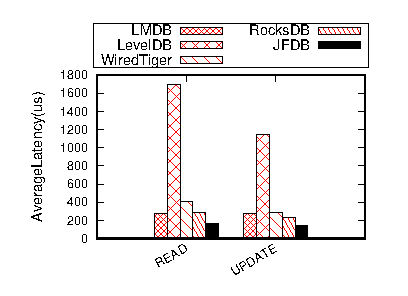
\includegraphics[width=0.24\textwidth]{./ycsb_graph/ycsb_16_a.eps}
	}
    \subfloat[Webserver]{
        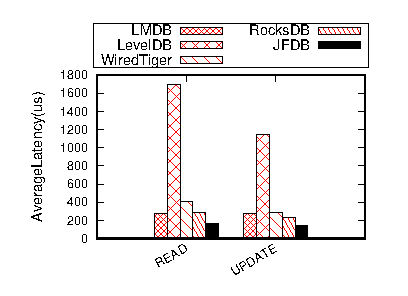
\includegraphics[width=0.24\textwidth]{./ycsb_graph/ycsb_16_a.eps}
	} 
    \subfloat[Linkbench]{
        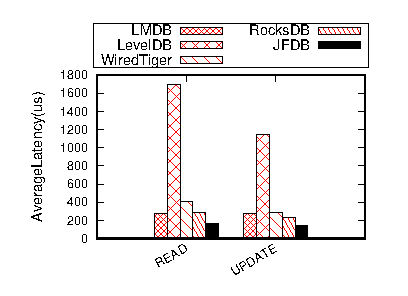
\includegraphics[width=0.24\textwidth]{./ycsb_graph/ycsb_16_a.eps}
	}
	\subfloat[YCSB-00]{
        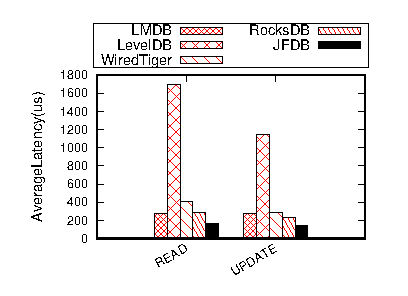
\includegraphics[width=0.24\textwidth]{./ycsb_graph/ycsb_16_a.eps}
	} \\
	\subfloat[YCSB-01]{
        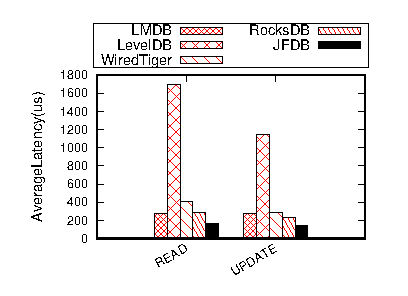
\includegraphics[width=0.24\textwidth]{./ycsb_graph/ycsb_16_a.eps}
	} 
	\subfloat[Systor-16LUN3]{
        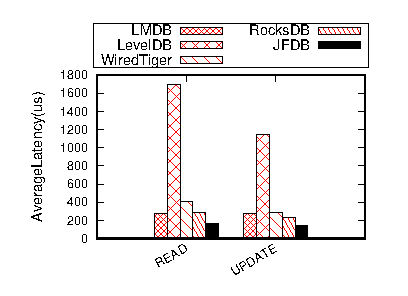
\includegraphics[width=0.24\textwidth]{./ycsb_graph/ycsb_16_a.eps}
	} 
	\subfloat[Systor-16LUN4]{
        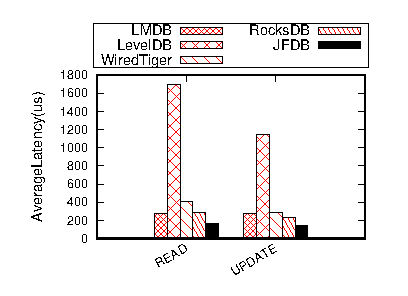
\includegraphics[width=0.24\textwidth]{./ycsb_graph/ycsb_16_a.eps}
	} 
	\subfloat[Systor-18LUN3]{
        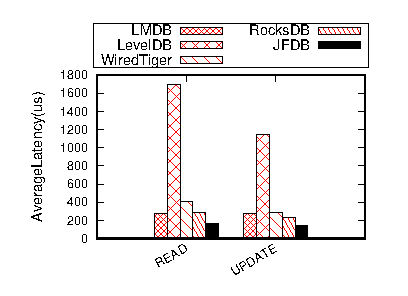
\includegraphics[width=0.24\textwidth]{./ycsb_graph/ycsb_16_a.eps}
	} 

	\caption{\textbf{Hit ratio in protected mapping table pages.}
%		\st{The \texttt{fillrandom} inserts items with random keys for each thread,
%    and the \texttt{overwrite} updates existing values in random order.
%    Both represent a put operation.
%    The \texttt{readrandom} retrieves items randomly,
%    and the \texttt{seekrandom} performs random seeks and queries the next ten items.}
	 }\label{fig_hit_ratio}
\end{figure*} 



\begin{figure*}[!bt]
    \centering{}
    \subfloat[Fileserver]{
        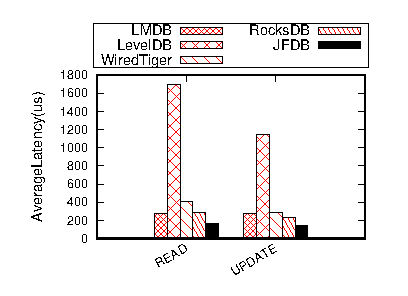
\includegraphics[width=0.24\textwidth]{./ycsb_graph/ycsb_16_a.eps}
	}
    \subfloat[Webserver]{
        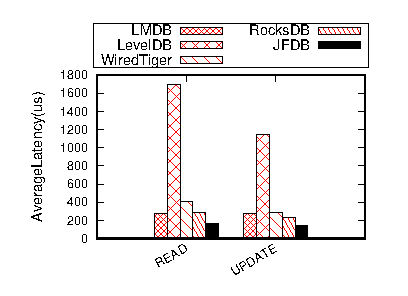
\includegraphics[width=0.24\textwidth]{./ycsb_graph/ycsb_16_a.eps}
	} 
    \subfloat[Linkbench]{
        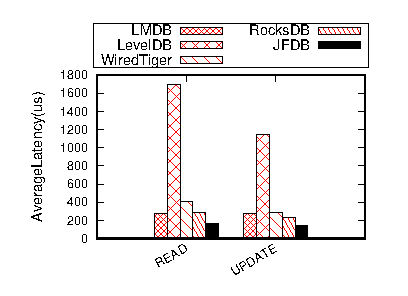
\includegraphics[width=0.24\textwidth]{./ycsb_graph/ycsb_16_a.eps}
	}
	\subfloat[YCSB-00]{
        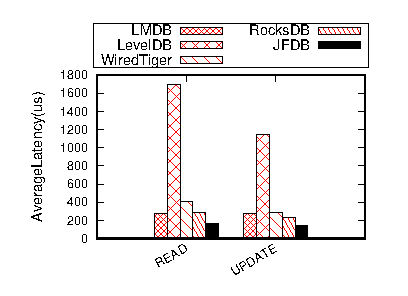
\includegraphics[width=0.24\textwidth]{./ycsb_graph/ycsb_16_a.eps}
	} \\
	\subfloat[YCSB-01]{
        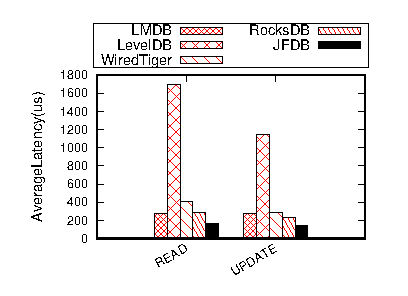
\includegraphics[width=0.24\textwidth]{./ycsb_graph/ycsb_16_a.eps}
	} 
	\subfloat[Systor-16LUN3]{
        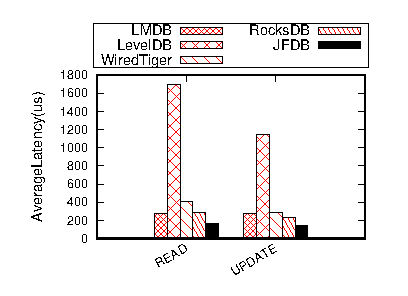
\includegraphics[width=0.24\textwidth]{./ycsb_graph/ycsb_16_a.eps}
	} 
	\subfloat[Systor-16LUN4]{
        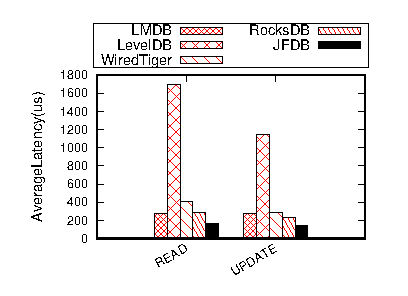
\includegraphics[width=0.24\textwidth]{./ycsb_graph/ycsb_16_a.eps}
	} 
	\subfloat[Systor-18LUN3]{
        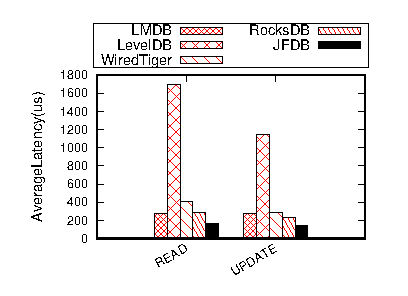
\includegraphics[width=0.24\textwidth]{./ycsb_graph/ycsb_16_a.eps}
	} 

	\caption{\textbf{Write-back traffic of mapping table.}
%		\st{The \texttt{fillrandom} inserts items with random keys for each thread,
%    and the \texttt{overwrite} updates existing values in random order.
%    Both represent a put operation.
%    The \texttt{readrandom} retrieves items randomly,
%    and the \texttt{seekrandom} performs random seeks and queries the next ten items.}
	 }\label{fig_write_traffic}
\end{figure*} 



%\begin{figure*}[t!]
\section{Design and Implementation}
\iffalse
This section describes the design and implementation of \ours{} buffer in detail. 
\S~\ref{subsec:overview} overviews the overall architecture of the in-storage buffer under capacitance constraints, and \S~\ref{subsec:lind_sched} presents the I/O scheduling algorithm
to reduce the write traffic in \ours{}.

\subsection{Overview}
\label{subsec:overview}
To satisfy a high demand for storage capacity in modern applications,
the SSDs have become highly scalable with advances in density-increasing techniques. 
The state-of-the-art SSDs provide tens of TBs capacity and this trend is expected 
to continue in the future.
The problem is that the capacitors, an integral component used in SSDs to protect the buffer data
in power outage, is unable to keep up with the significant density increase speed of NAND flash memory. 
The SSD-internal buffer is typically 0.1\% of the storage capacity in size.
To protect the entire buffer of SSD, the capacitors 
should have been improved at the same pace with SSD in density; 
its density has enhanced only at one-fifth speed of SSD density improvement. 
% This density gap between capacitors and memory technologies
% indicates that 
With this density gap, the PLP with full protection is no longer feasible in SSDs; 
it not only severely limits the form factor of SSDs requiring deployment of a large number of capacitors but also significantly increases the manufacturing cost of SSDs. 

\ours{} is designed to efficiently maintain the in-storage buffer under capacitance limitations. 
Table~\ref{tab:ssd_buff_comp} shows the breakdown of the in-storage buffer usage for each component
for 512GB SSD that has an architecture shown in Table~\ref{tab:ssd_config}. 
The user data buffer is employed to fully exploit the underlying flash parallelism.
Hence, it is typically twice the size of all pages that can be programmed in parallel, 
which is 4MB in this setting, while it may vary depending on the design choice. 
The mapping table that translates LPN(logical page number) to PPN(physical page number) 
accounts for 512MB, which corresponds to 97\% of the buffer size. 
Other metadata including mapping table directory uses a total of 10.5MB buffer. 

To overcome capacitance constraints for SSD, \ours{} sacrifices on some durability of mapping table, 
% by only protecting a portion of it, 
while protecting the user data and the metadata other than mapping table with capacitors. 
The user data persistence should be synchronously guaranteed with the host request
to conserve the properties of existing SSDs with PLP. 
For this reason, making a compromise on it can lead to a serious performance penalty in SSD.
On contrary, the requirements for the mapping table update are less stringent;
it does not have to be immediate upon a host request because the address translation is 
necessary only when the associated data is actually programmed to the flash memory. 
This nature allows a room for reasonable trade-off between capacitance and performance,
by effectively maintaining the persisting overhead of mapping table under capacitance constraint. 
Other metadata updates are also asynchronous with the host request, but
they use only a marginal space of the buffer; sophisticating their management mechanism 
for further capacitance saving is cost-ineffective. 

% because the PPN of data is determined when it is flushed to the flash memory. 
% The LPB to PPN translation is required when the data is in flash memory. 
% it can be restored on the reboot. 

% 요청된 데이터를 찾기 위해 사용. 
% 데이터는 보호되고 있는데 인덱스는 잃어버림. 
% ==> 추후 recovery 할 때 반영해주면 됨. 데이터를 쓰면서 업데이트 하거나 '
% ==> 이미 데이터가 플래시에 쓰여져 있다면? 걔는 보호를 해줘야 함. 
% ==> 대신 small write 임. 버퍼링 효과를 늘리면 footprint 를 줄일 수 있음. 

\iffalse
If an SSD has 8 channels and 4 ways per channel with 8KB page size, about 128KB of memory (twicethe  size  of  all  pages  that  can  be  written  in  parallel)  are  usedfor data buffering. This, however, only accounts for 0.02% ofthe volatile DRAM.
maximize the high degree of parallism in SSDs 
during the operation of flash memories 
\fi

% the end of full protection based SSD design 
%The capacitance faces scaling limit 

% mapping table 이 상당히 큰 부분을 차지한다. 
% 사용자 버퍼는 통상 SSD의 병렬성을 활용할 수 있는 정도로만 있으면 된다고 했지만, 
% 최근 다양한 이유로 증가하고 있음. 

\subsection{Least Increase of Dirtiness Scheduling}
\label{subsec:lind_sched}
\fi
\ours{} partially protects the mapping table with limited capacitance. 
When the dirty pages of mapping table become more than the maximum number of protected pages, 
\ours{} flushes them to flash memory based on the LRU (Least-recently Used) algorithm. 
Because this flush operation does not arise with SSD using PLP, mitigating the effect of this overhead 
is a key strategy to achieving high performance under capacitance constraints. 
To this end, \ours{} presents a cost-effective scheduling scheme for the in-storage buffer.
\ours{} prefers to force the user data that increases the dirtiness of the mapping 
table the least to flash memory. This scheme reduces the dirty page footprint 
of the mapping table at a time window by enhancing the locality of updates. 
As a result, the frequency of flush operation for the mapping table can be 
largely reduced. 

\begin{figure}
    \centering{}
    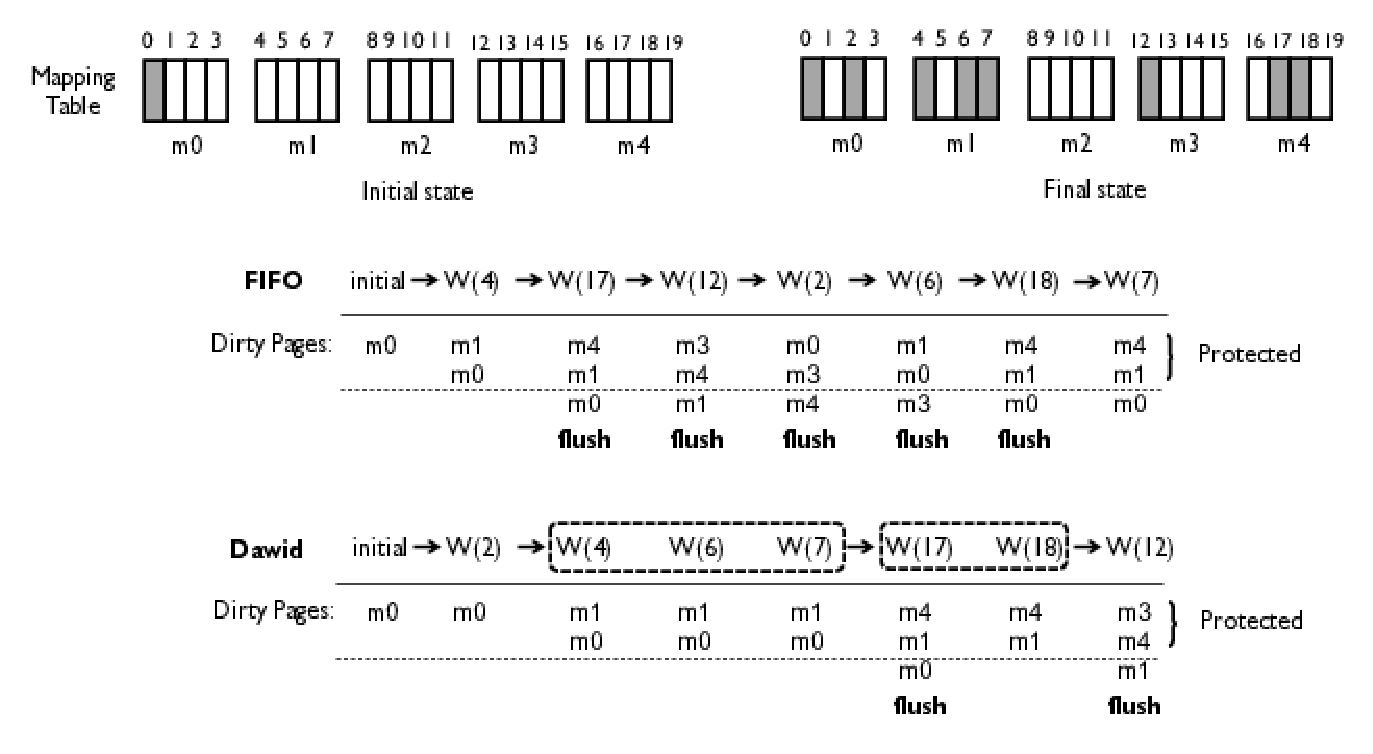
\includegraphics[width=0.5\textwidth]{figure/dawid_algo.eps}
    \caption{\textbf{\ours{}-SSD buffer management scheme}}
    \label{fig:dawid_buff_overview}
\end{figure}


Figure~\ref{fig:dawid_buff_overview} compares the flush overhead of \texttt{FIFO} and \ours{} scheduling in SSD buffer. 
In this example, there are seven write requests 
in the device queue, sent from host in the following order: \texttt{W(4)}, \texttt{W(17)}, \texttt{W(12)}, \texttt{W(2)}, \texttt{W(6)}, \texttt{W(18)}, and \texttt{W(7)}.  
The mapping table has one dirty page (\texttt{m0}) 
at an initial state. We assume that 2 out of 5 pages of the mapping table are protected. 
FIFO writes the user data in the buffer to flash memory in arrival order. 
With this scheme, the mapping table would be randomly updated, generating a large number of dirty pages at a 
time window. 
Consequently, FIFO incurs a total of five flushes of the mapping table page during the write process. 


In contrast, \ours{} calculates the write cost for each data that indicates an
increase in the number of dirty pages of the mapping table when it is flushed,
and it processes the request with minimum cost first.  In this example, the
write request \texttt{W(2)} has a top priority because its associated mapping
table page (\texttt{m0}) is already dirty, and thus it does not add the dirty
pages of the mapping table.  Next, the write requests \texttt{W(4)},
\texttt{W(6)}, and \texttt{W(7)} are processed.  Because their address mapping
entries are located in the same page of the mapping table, the cost of flushing
them is reduced to one third.  With this scheme, \ours{} can reduce the footprint
of mapping table updates within time intervals, thereby delivering only two
flushes of the mapping table for the same task. 

\iffalse
\subsection{Eviction Policy}
\begin{figure}[t!]
    \centering{}
	\subfloat[JESD] { 
    	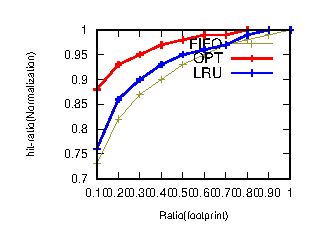
\includegraphics[width=0.2\textwidth]{expr/hitMap/eps/JESD_FIFO.eps}
    	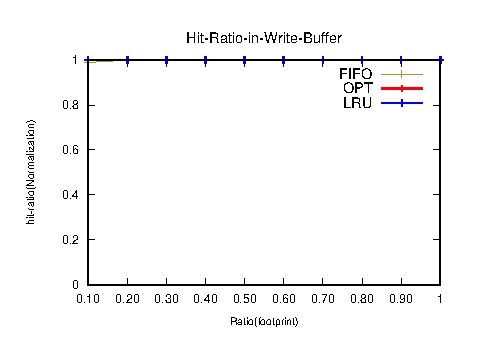
\includegraphics[width=0.2\textwidth]{expr/hitMap/eps/JESD_DAWID.eps}
	} \\
	\subfloat[OLTP]{ 
    	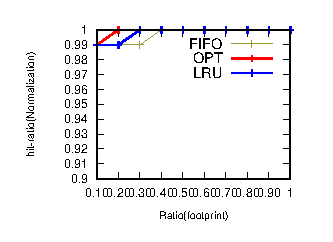
\includegraphics[width=0.2\textwidth]{expr/hitMap/eps/OLTP_FIFO.eps}
    	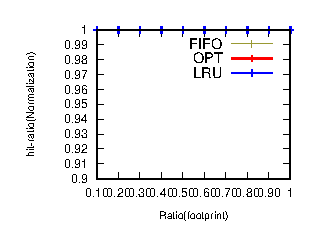
\includegraphics[width=0.2\textwidth]{expr/hitMap/eps/OLTP_DAWID.eps}
	} \\
	\subfloat[Linkbench]{ 
    	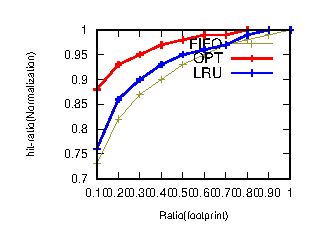
\includegraphics[width=0.2\textwidth]{expr/hitMap/eps/JESD_FIFO.eps}
    	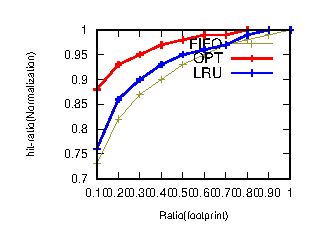
\includegraphics[width=0.2\textwidth]{expr/hitMap/eps/JESD_FIFO.eps}
	} \\
    \caption{\textbf{Write hit ratio for the protected range in a mapping table.}}
    \label{fig_dawid_archi}
\end{figure}
\fi

% \section{Implementation}
We implement \ours{} in \texttt{FEMU}, an open-source SSD development
framework~\cite{li2018case}. Fig.~\ref{fig_dawid_archi} shows the overall
architecture of \ours{}-SSD and its internal data structures. As the original
version of \texttt{FEMU} directly writes data to flash memories without write
buffering, we extend it to use a small-sized write buffer, which aggregates and  
batches user writes into the underlying flash memory.  

\ours{}-SSD maintains three different threads that are executing concrrently
within SSDs.  The \texttt{nvm\_poller} takes a charge of transferring requests
between NVMe queues and FTL-internal queues. The FTL-internal queue consists of
a pair of sub-queues, each of which is named \texttt{to\_ftl} and
\texttt{to\_poller}). This separation is intended to enable a non-blocking
access to queues by allowing only a single writer for each queue.  Second, the
\texttt{ftl\_thread} essentially handles the ingress requests from the internal
queues. For write, it transfers data from the host memory to the SSD-internal
write buffer with DMA and updates the associated entry in a translation page to
point to the write buffer. Then, it notifies the completion of request to the
\texttt{nvm\_poller} by enqueueing the acknowledgement into the
\texttt{to\_poller} queue.  Because \ours{} protects the entire space of write
buffer with capacitance, data persistency is guaranteed for all acknowledged
writes.  For read, the \texttt{ftl\_thread} retrieves the requested data by
consulting the mapping table and transfers it to the host. 

The \texttt{ftl\_flush\_thread} plays a role of writing data from a DRAM-buffer
into a flash memory.  With the \texttt{FIFO} policy, the user writes are issued
to NAND flash memory in the order they arrive into the buffer. However, \ours{}
flushes buffered writes in the order such that it least increases the dirty memory
footprint of the mapping table.  To realize this design, \ours{} maintains two
data structures, as depicted in Fig.~\ref{fig_dawid_archi}(b). First, \textit{a
zero-cost list} that holds the indexes to tranlsation pages that is already
in a dirty state, and second, \textit{a max binary heap} that
maintains the indexes to translation pages sorted by the number of buffered
user write requests associated with that page.  

%When there is sufficient bandwidth at underlying NAND flash subsystem for writes, 
When a half of the write buffer becomes occupied, flushing is invoked. \ours{}-SSD
first flushes user data whose translation pages in the zero-cost list, and then
persists user data as their translation pages are ordered by the max binary
heap. By doing so, each user write minimizes the number of eventual
translation page write, and each translation page write maximizes the number of
persisted mapping entries. These data structures are updated by the \texttt{ftl\_thread} 
when a write request arrives at SSD. 
To exploit the SSD internal parallelism, we send data to flash memory in
batches by the number of NAND flash chips that can be written simultaneously.

Once the write operations of NAND flash memory complete,
\texttt{ftl\_flush\_thread} updates the mapping table entries to point to the
physical address of the data in a flash memory.  At this moment, if the number
of dirty mapping table pages goes beyond the protectable number of pages,
\texttt{ftl\_flush\_thread} persists the mapping table page to flash memory.
This is also conducted in batches by the number of NAND flash chips that can be
written in parallel.

\section{Implementation}
\begin{figure}[t!]
    \centering{}
	\subfloat[Architecture] { 
    	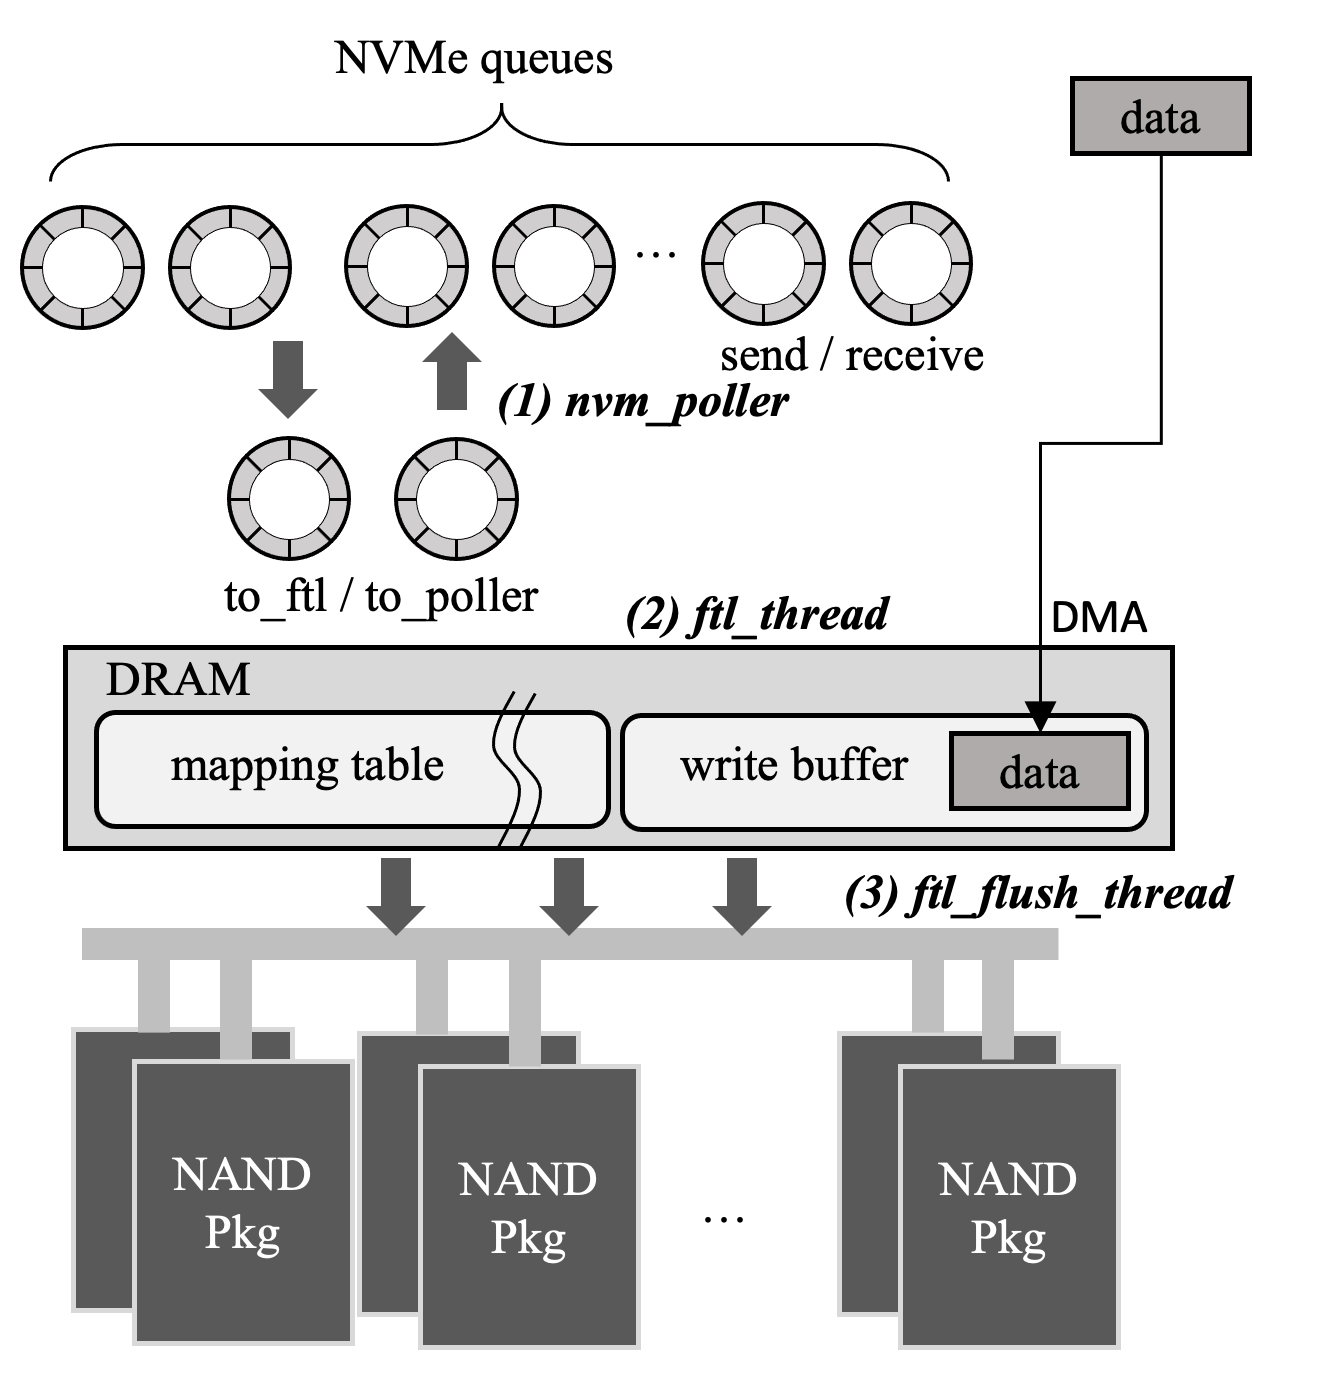
\includegraphics[width=0.3\textwidth]{figure/dawid_ssd_archi_new.eps}
	} \\
	\subfloat[Data structures for FTL]{ 
    	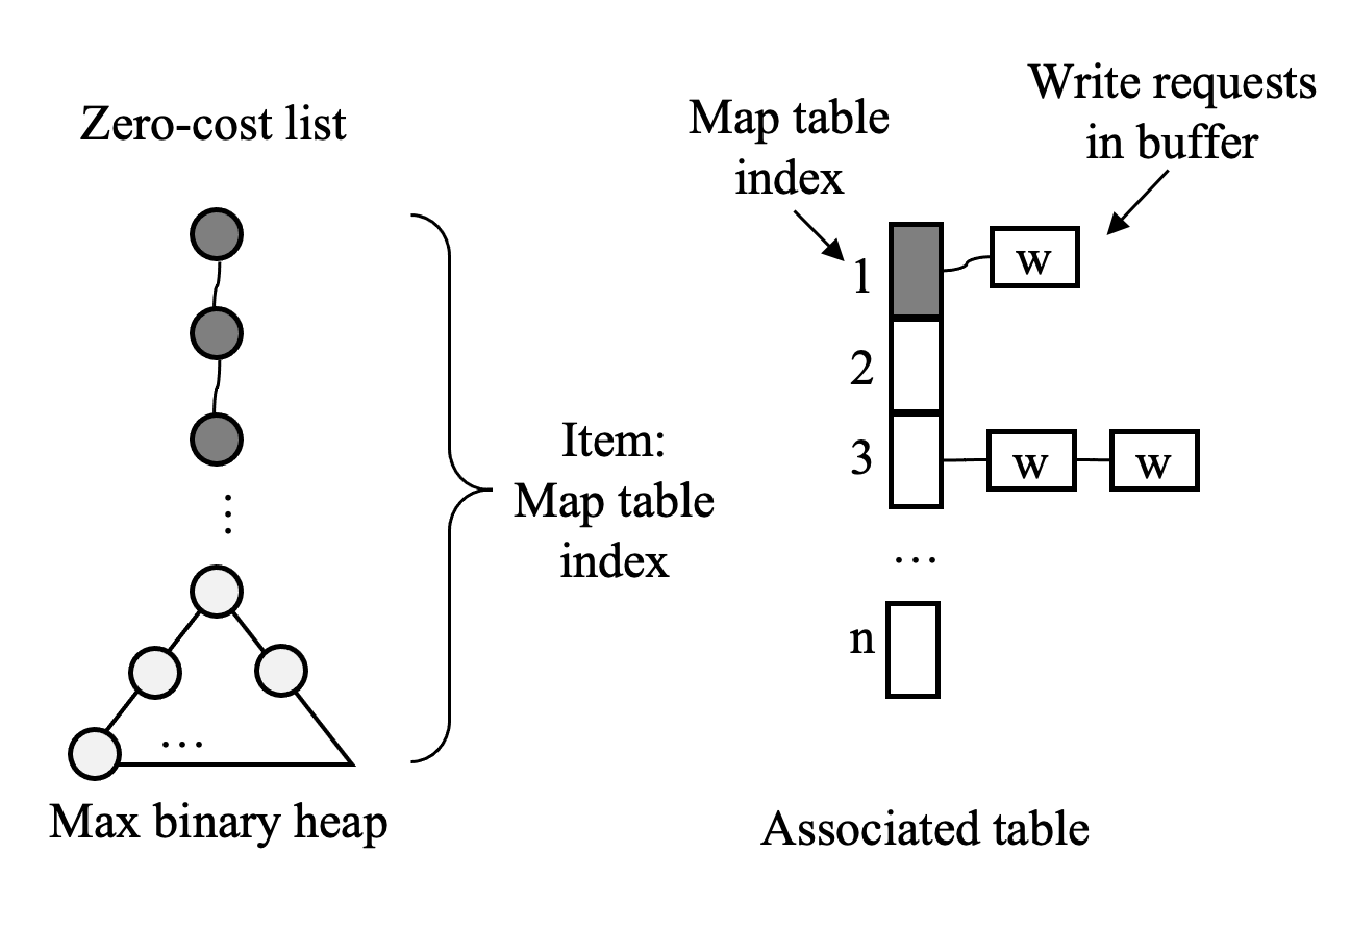
\includegraphics[width=0.4\textwidth]{figure/dawid_ds.eps}
	}

    %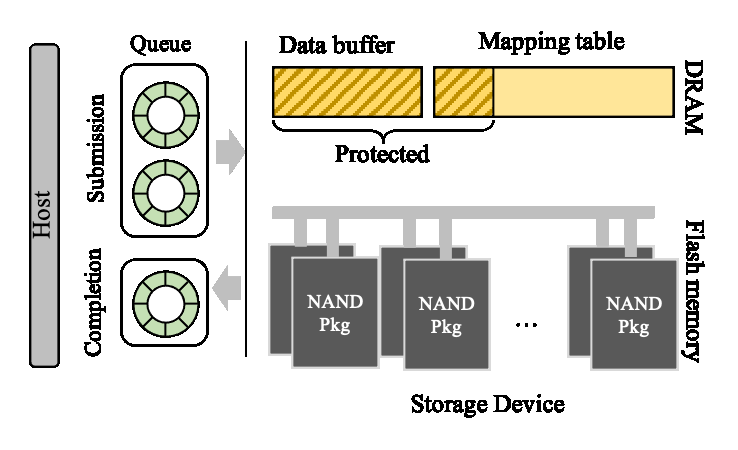
\includegraphics[width=0.4\textwidth]{figure/dawid_ssd_archi.eps}
    \caption{\textbf{Dawid-SSD}}
    \label{fig_dawid_archi}
\end{figure}


\begin{figure*}[!t]
    \centering{}
	\subfloat[Random] { 
	    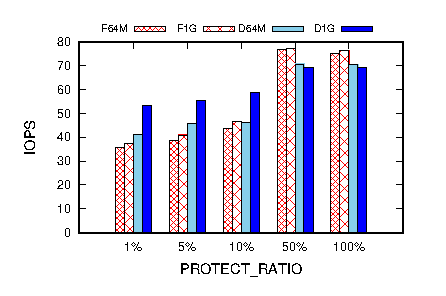
\includegraphics[width=0.3\textwidth]{expr/micro_rslt_220525/perf/perf_RAND.eps}
	} 
	\subfloat[JESD] { 
	    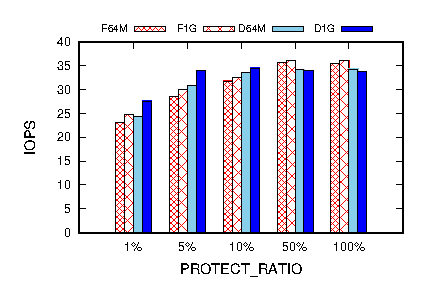
\includegraphics[width=0.3\textwidth]{expr/micro_rslt_220525/perf/perf_JESD.eps}
	}
	\subfloat[TPC-C] { 
	    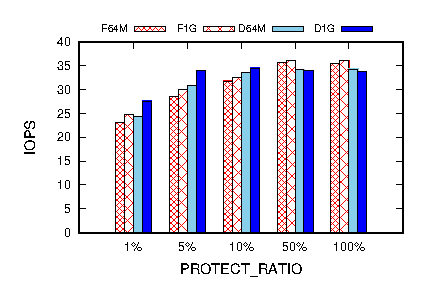
\includegraphics[width=0.3\textwidth]{expr/micro_rslt_220525/perf/perf_JESD.eps}
	}

    \caption{\textbf{IOPS}}
\end{figure*} 


\begin{figure*}[!t]
    \centering{}
	\subfloat[Random] { 
	    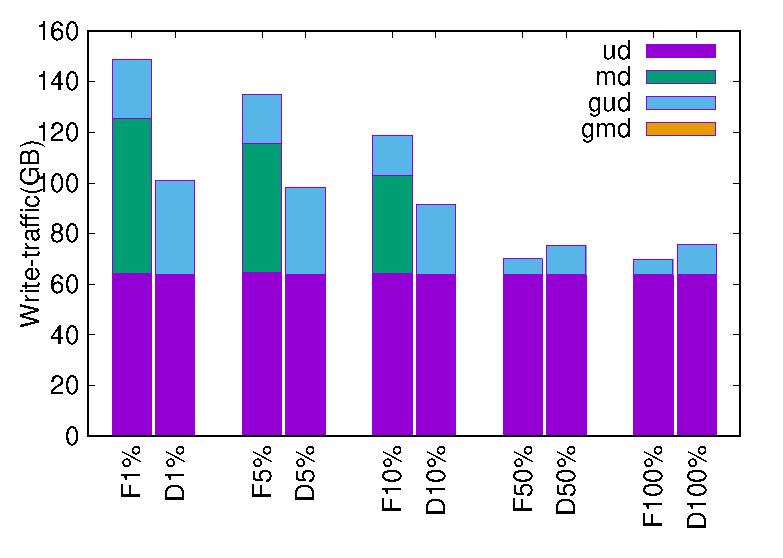
\includegraphics[width=0.3\textwidth]{expr/micro_rslt_220525/wt/RAND_1.eps}
	} 
	\subfloat[JESD] { 
	    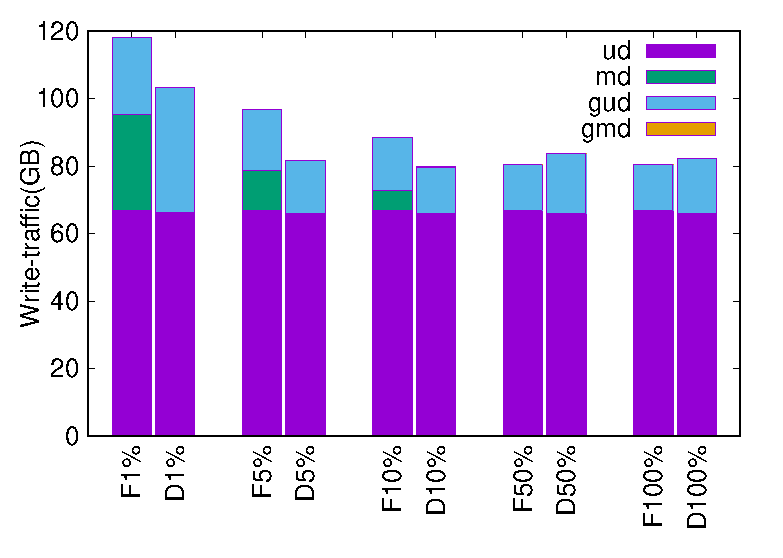
\includegraphics[width=0.3\textwidth]{expr/micro_rslt_220525/wt/JESD_1.eps}
	}
	\subfloat[TPC-C] { 
	    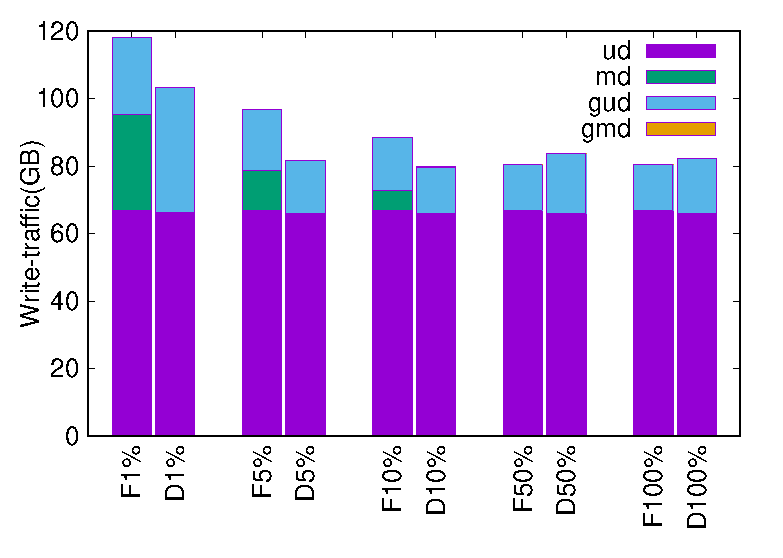
\includegraphics[width=0.3\textwidth]{expr/micro_rslt_220525/wt/JESD_1.eps}
	}
    \caption{\textbf{Write Traffic.}}
\end{figure*} 



We implement \ours{} in \texttt{FEMU}, an open-source SSD development
framework~\cite{li2018case}. Fig.~\ref{fig_dawid_archi} shows the overall
architecture of \ours{}-SSD and its internal data structures. As the original
version of \texttt{FEMU} directly writes data to flash memories without write
buffering, we extend it to use a small-sized write buffer, which aggregates and  
batches user writes into the underlying flash memory.  

\ours{}-SSD maintains three different threads that are executing concrrently
within SSDs.  The \texttt{nvm\_poller} takes a charge of transferring requests
between NVMe queues and FTL-internal queues. The FTL-internal queue consists of
a pair of sub-queues, each of which is named \texttt{to\_ftl} and
\texttt{to\_poller}). This separation is intended to enable a non-blocking
access to queues by allowing only a single writer for each queue.  Second, the
\texttt{ftl\_thread} essentially handles the ingress requests from the internal
queues. For write, it transfers data from the host memory to the SSD-internal
write buffer with DMA and updates the associated entry in a translation page to
point to the write buffer. Then, it notifies the completion of request to the
\texttt{nvm\_poller} by enqueueing the acknowledgement into the
\texttt{to\_poller} queue.  Because \ours{} protects the entire space of write
buffer with capacitance, data persistency is guaranteed for all acknowledged
writes.  For read, the \texttt{ftl\_thread} retrieves the requested data by
consulting the mapping table and transfers it to the host. 

The \texttt{ftl\_flush\_thread} plays a role of writing data from a DRAM-buffer
into a flash memory.  With the \texttt{FIFO} policy, the user writes are issued
to NAND flash memory in the order they arrive into the buffer. However, \ours{}
flushes buffered writes in the order such that it least increases the dirty memory
footprint of the mapping table.  To realize this design, \ours{} maintains two
data structures, as depicted in Fig.~\ref{fig_dawid_archi}(b). First, \textit{a
zero-cost list} that holds the indexes to tranlsation pages that is already
in a dirty state, and second, \textit{a max binary heap} that
maintains the indexes to translation pages sorted by the number of buffered
user write requests associated with that page.  

%When there is sufficient bandwidth at underlying NAND flash subsystem for writes, 
When a half of the write buffer becomes occupied, flushing is invoked. \ours{}-SSD
first flushes user data whose translation pages in the zero-cost list, and then
persists user data as their translation pages are ordered by the max binary
heap. By doing so, each user write minimizes the number of eventual
translation page write, and each translation page write maximizes the number of
persisted mapping entries. These data structures are updated by the \texttt{ftl\_thread} 
when a write request arrives at SSD. 
To exploit the SSD internal parallelism, we send data to flash memory in
batches by the number of NAND flash chips that can be written simultaneously.

Once the write operations of NAND flash memory complete,
\texttt{ftl\_flush\_thread} updates the mapping table entries to point to the
physical address of the data in a flash memory.  At this moment, if the number
of dirty mapping table pages goes beyond the protectable number of pages,
\texttt{ftl\_flush\_thread} persists the mapping table page to flash memory.
This is also conducted in batches by the number of NAND flash chips that can be
written in parallel.


\section{Evaluation}
%We assume 1\% of the mapping table is protected via capacitors in a 64GB SSD. 
%The 64GB SSD is using DRAM and assumes that 1\% of the mapping table is
%protected. 
We perform the experiments on a machine with a 20-core Intel Xeon(R) Silver
4114 CPU running at 2.2GHz and 84GB memory. We run FEMU (QEMU-based SSD
emulator) configured to use 10 cores, 4GB DRAM for main memory, and 16GB DRAM
for SSD emulation. The SSD maintains a mapping table entirely in DRAM partially 
protected with capacitance.

We measure the average IOPS and write traffic varying the protected ratio of
the mapping table from 1\% to 100\%. We study two different size of write
buffers, which are 64MB and 1GB, respectively. 
We use two benchmarks for \ours{} performance evaluation. Using the fio
benchmark~\cite{fio-bench}, we generate two kinds of workloads: the 4KB of
random writes (denoted as RANDOM) and the skewed read-write mixed workload that follows JESD219 (JESD)
using 8 threads.  A total of 90GB of data was written to the 30GB area.



%\begin{figure*}[t]
%    \centering{}
%	\subfloat[OLTP] { 
%	    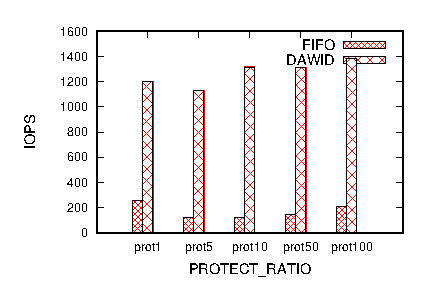
\includegraphics[width=0.3\textwidth]{expr/macro_220517/perf/OLTP/perf_OLTP.eps}
%	} 
%	\subfloat[Write Traffic] { 
%	    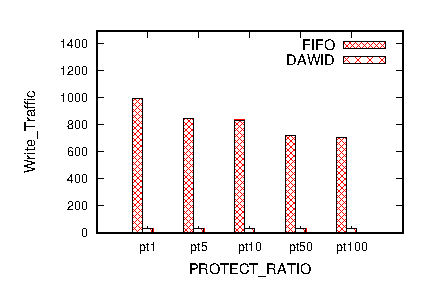
\includegraphics[width=0.3\textwidth]{expr/macro_220517/wt/OLTP/perf_OLTP.eps}
%	} 
%    \caption{\textbf{OLTP}}
%\end{figure*} 



%\begin{figure*}[t]
%    \centering{}
%	\subfloat[Sequential] { 
%	    %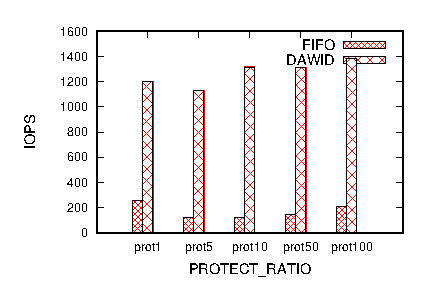
\includegraphics[width=0.3\textwidth]{expr/macro_220517/perf/OLTP/perf_OLTP.eps}
%	    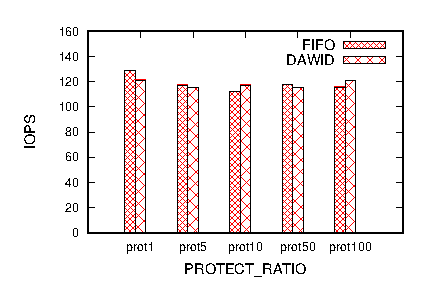
\includegraphics[width=0.3\textwidth]{expr/micro_220517/perf/SEQ/perf_SEQ.eps}
%	} 
%	\subfloat[Random] { 
%	    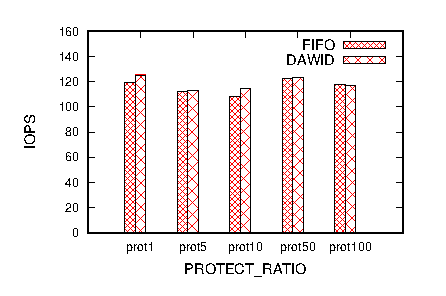
\includegraphics[width=0.3\textwidth]{expr/micro_220517/perf/RAND/perf_RAND.eps}
%	} 
%	\subfloat[JESD] { 
%	    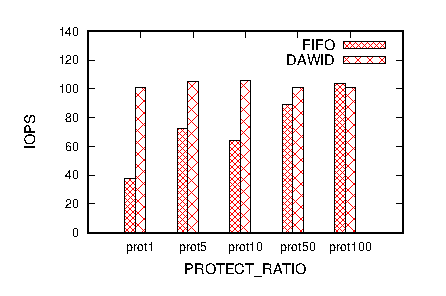
\includegraphics[width=0.3\textwidth]{expr/micro_220517/perf/JESD/perf_JESD.eps}
%	}
%    \caption{\textbf{IOPS}}
%\end{figure*} 
%




\section{Conclusion}
In this paper, we present Hexa's design, implementation, 
and evaluation to reduce performance overhead due to metadata flush in 
a situation where PLP is partially supported on enterprise-class SSDs. 
Our desing operates using only a small amount of Capacitor's capacity compared
to the previous one. It also minimizes the impact of metadata by buffering requests using the 
scalability of the write buffer. 
Our evaluation results show that Hexa improves performance in situations where requests are randomly generated. 
In addition, JESD and real-benchmark results comfirm that there are advantages in a real-world environment.





\bibliographystyle{plain}
\bibliography{dawid_fast}


%\theendnotes

\end{document}







